

\tikzset{every picture/.style={line width=0.3pt}} %set default line width to 0.75pt        

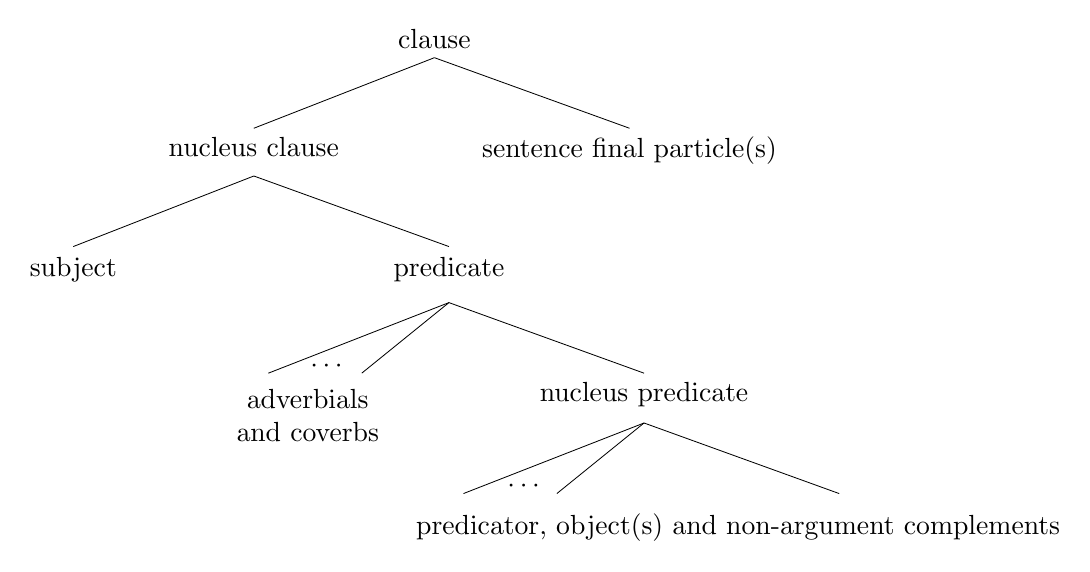
\begin{tikzpicture}[x=0.75pt,y=0.75pt,yscale=-1,xscale=1]
%uncomment if require: \path (0,383); %set diagram left start at 0, and has height of 383

%Straight Lines [id:da03870203201071365] 
\draw    (306,64.48) -- (219,98.48) ;
%Straight Lines [id:da09410121434078333] 
\draw    (306,64.48) -- (400,98.48) ;
%Straight Lines [id:da6473752338850502] 
\draw    (219,121.48) -- (132,155.48) ;
%Straight Lines [id:da22452164165522825] 
\draw    (219,121.48) -- (313,155.48) ;
%Straight Lines [id:da12042747516750363] 
\draw    (313,182.48) -- (226,216.48) ;
%Straight Lines [id:da6837235841990796] 
\draw    (313,182.48) -- (407,216.48) ;
%Straight Lines [id:da3234320748825805] 
\draw    (313,182.48) -- (271,216.48) ;
%Straight Lines [id:da4586272779304892] 
\draw    (407,240.48) -- (320,274.48) ;
%Straight Lines [id:da815197318792398] 
\draw    (407,240.48) -- (501,274.48) ;
%Straight Lines [id:da0031789117644716036] 
\draw    (407,240.48) -- (365,274.48) ;

% Text Node
\draw (306,61.48) node [anchor=south] [inner sep=0.75pt]   [align=left] {clause};
% Text Node
\draw (400,101.48) node [anchor=north] [inner sep=0.75pt]   [align=left] {sentence final particle(s)};
% Text Node
\draw (219,101.48) node [anchor=north] [inner sep=0.75pt]   [align=left] {nucleus clause};
% Text Node
\draw (132,159.48) node [anchor=north] [inner sep=0.75pt]   [align=left] {subject};
% Text Node
\draw (313,159.48) node [anchor=north] [inner sep=0.75pt]   [align=left] {predicate};
% Text Node
\draw (245,209) node [anchor=north west][inner sep=0.75pt]   [align=left] {$\displaystyle \cdots $};
% Text Node
\draw (207,223) node [anchor=north west][inner sep=0.75pt]   [align=left] {\begin{minipage}[lt]{55.17pt}\setlength\topsep{0pt}
\begin{center}
adverbials\\and coverbs
\end{center}

\end{minipage}};
% Text Node
\draw (407,219.48) node [anchor=north] [inner sep=0.75pt]   [align=left] {nucleus predicate};
% Text Node
\draw (340,267) node [anchor=north west][inner sep=0.75pt]   [align=left] {$\displaystyle \cdots $};
% Text Node
\draw (296,283) node [anchor=north west][inner sep=0.75pt]   [align=left] {predicator, object(s) and non-argument complements};


\end{tikzpicture}
